%!TEX program = xelatex+makeindex+bibtex
\documentclass[final]{scrreprt} %scrreprt of scrartcl
% Include all project wide packages here.
\usepackage{fullpage}
\usepackage{polyglossia}
\setmainlanguage{english}
\usepackage{csquotes}
\usepackage{graphicx}
\usepackage{epstopdf}
\usepackage{pdfpages}
\usepackage{caption}
\usepackage[list=true]{subcaption}
\usepackage{float}
\usepackage{standalone}
\usepackage{import}
\usepackage{tocloft}
\usepackage{wrapfig}
\usepackage{authblk}
\usepackage{array}
\usepackage{booktabs}
\usepackage[toc,page,title,titletoc]{appendix}
\usepackage{xunicode}
\usepackage{fontspec}
\usepackage{pgfplots}
\usepackage{SIunits}
\usepackage{units}
\pgfplotsset{compat=newest}
\pgfplotsset{plot coordinates/math parser=false}
\newlength\figureheight 
\newlength\figurewidth
\usepackage{amsmath}
\usepackage{mathtools}
\usepackage{unicode-math}
\usepackage[
    backend=bibtexu,
	texencoding=utf8,
bibencoding=utf8,
    style=ieee,
    sortlocale=en_US,
    language=auto
]{biblatex}
\usepackage{listings}
\newcommand{\includecode}[3][c]{\lstinputlisting[caption=#2, escapechar=, style=#1]{#3}}
\newcommand{\superscript}[1]{\ensuremath{^{\textrm{#1}}}}
\newcommand{\subscript}[1]{\ensuremath{_{\textrm{#1}}}}


\newcommand{\chapternumber}{\thechapter}
\renewcommand{\appendixname}{Bijlage}
\renewcommand{\appendixtocname}{Bijlagen}
\renewcommand{\appendixpagename}{Bijlagen}

\usepackage[hidelinks]{hyperref} %<--------ALTIJD ALS LAATSTE

\renewcommand{\familydefault}{\sfdefault}

\setmainfont[Ligatures=TeX]{Myriad Pro}
\setmathfont{Asana Math}
\setmonofont{Lucida Console}

\usepackage{titlesec, blindtext, color}
\definecolor{gray75}{gray}{0.75}
\newcommand{\hsp}{\hspace{20pt}}
\titleformat{\chapter}[hang]{\Huge\bfseries}{\chapternumber\hsp\textcolor{gray75}{|}\hsp}{0pt}{\Huge\bfseries}
\renewcommand{\familydefault}{\sfdefault}
\renewcommand{\arraystretch}{1.2}
\setlength\parindent{0pt}

%For code listings
\definecolor{black}{rgb}{0,0,0}
\definecolor{browntags}{rgb}{0.65,0.1,0.1}
\definecolor{bluestrings}{rgb}{0,0,1}
\definecolor{graycomments}{rgb}{0.4,0.4,0.4}
\definecolor{redkeywords}{rgb}{1,0,0}
\definecolor{bluekeywords}{rgb}{0.13,0.13,0.8}
\definecolor{greencomments}{rgb}{0,0.5,0}
\definecolor{redstrings}{rgb}{0.9,0,0}
\definecolor{purpleidentifiers}{rgb}{0.01,0,0.01}


\lstdefinestyle{csharp}{
language=[Sharp]C,
showspaces=false,
showtabs=false,
breaklines=true,
showstringspaces=false,
breakatwhitespace=true,
escapeinside={(*@}{@*)},
columns=fullflexible,
commentstyle=\color{greencomments},
keywordstyle=\color{bluekeywords}\bfseries,
stringstyle=\color{redstrings},
identifierstyle=\color{purpleidentifiers},
basicstyle=\ttfamily\small}

\lstdefinestyle{c}{
language=C,
showspaces=false,
showtabs=false,
breaklines=true,
showstringspaces=false,
breakatwhitespace=true,
escapeinside={(*@}{@*)},
columns=fullflexible,
commentstyle=\color{greencomments},
keywordstyle=\color{bluekeywords}\bfseries,
stringstyle=\color{redstrings},
identifierstyle=\color{purpleidentifiers},
}

\lstdefinestyle{matlab}{
language=Matlab,
showspaces=false,
showtabs=false,
breaklines=true,
showstringspaces=false,
breakatwhitespace=true,
escapeinside={(*@}{@*)},
columns=fullflexible,
commentstyle=\color{greencomments},
keywordstyle=\color{bluekeywords}\bfseries,
stringstyle=\color{redstrings},
identifierstyle=\color{purpleidentifiers}
}

\lstdefinestyle{vhdl}{
language=VHDL,
showspaces=false,
showtabs=false,
breaklines=true,
showstringspaces=false,
breakatwhitespace=true,
escapeinside={(*@}{@*)},
columns=fullflexible,
commentstyle=\color{greencomments},
keywordstyle=\color{bluekeywords}\bfseries,
stringstyle=\color{redstrings},
identifierstyle=\color{purpleidentifiers}
}

\lstdefinestyle{xaml}{
language=XML,
showspaces=false,
showtabs=false,
breaklines=true,
showstringspaces=false,
breakatwhitespace=true,
escapeinside={(*@}{@*)},
columns=fullflexible,
commentstyle=\color{greencomments},
keywordstyle=\color{redkeywords},
stringstyle=\color{bluestrings},
tagstyle=\color{browntags},
morestring=[b]",
  morecomment=[s]{<?}{?>},
  morekeywords={xmlns,version,typex:AsyncRecords,x:Arguments,x:Boolean,x:Byte,x:Char,x:Class,x:ClassAttributes,x:ClassModifier,x:Code,x:ConnectionId,x:Decimal,x:Double,x:FactoryMethod,x:FieldModifier,x:Int16,x:Int32,x:Int64,x:Key,x:Members,x:Name,x:Object,x:Property,x:Shared,x:Single,x:String,x:Subclass,x:SynchronousMode,x:TimeSpan,x:TypeArguments,x:Uid,x:Uri,x:XData,Grid.Column,Grid.ColumnSpan,Click,ClipToBounds,Content,DropDownOpened,FontSize,Foreground,Header,Height,HorizontalAlignment,HorizontalContentAlignment,IsCancel,IsDefault,IsEnabled,IsSelected,Margin,MinHeight,MinWidth,Padding,SnapsToDevicePixels,Target,TextWrapping,Title,VerticalAlignment,VerticalContentAlignment,Width,WindowStartupLocation,Binding,Mode,OneWay,xmlns:x}
}

%defaults
\lstset{
basicstyle=\ttfamily\small,
extendedchars=false,
numbers=left,
numberstyle=\ttfamily\tiny,
stepnumber=1,
tabsize=4,
numbersep=5pt
}
\addbibresource{../../library/bibliography.bib}
\usepackage{amsmath}
\usepackage{graphicx}
\title{Module 3 - Report}
\author{Alex {Misdorp} \and Sander {van Dijk}}
\begin{document}

\chapter{Assignment 2}
\section*{Task 3: Identifying the models' parameters}

Now that a model has been constructed we need to find the values for our A and B matrix. To find these we sent the car a signal and measured the output of the ultrasound sensors. In figure \ref{fig:KITT-input-output-model} the results are on display.
The blue signal represents the input signal and periodically goes above $x=0$ and beneath it. In between those transitions there will be a small delay where the input remains zero for a while. The model output will react accordingly whereby the postion increases for a positive input and decreases for a negative input.
The output signal from KITT shows a phase shift which might be contributed to the car's acceleration that is not instantaneous, there will be a certain delay. The jerking of the red line might also be contributed to this.

\begin{figure}[H]
	\centering
    	\setlength\figureheight{4cm}
    	\setlength\figurewidth{0.8\linewidth}
    	% This file was created by matlab2tikz v0.4.6 running on MATLAB 8.3.
% Copyright (c) 2008--2014, Nico Schlömer <nico.schloemer@gmail.com>
% All rights reserved.
% Minimal pgfplots version: 1.3
% 
% The latest updates can be retrieved from
%   http://www.mathworks.com/matlabcentral/fileexchange/22022-matlab2tikz
% where you can also make suggestions and rate matlab2tikz.
% 
\begin{tikzpicture}

\begin{axis}[%
width=\figurewidth,
height=\figureheight,
scale only axis,
xmin=0,
xmax=20,
xlabel={t (s)},
ymin=-250,
ymax=200,
ylabel={x (cm)},
legend style={at={(0.01,0.01)},anchor=south west,draw=black,fill=white,legend cell align=left}
]
\addplot [color=blue,solid]
  table[row sep=crcr]{
0	0	\\
0.1	0	\\
0.2	0	\\
0.3	0	\\
0.4	0	\\
0.5	0	\\
0.6	0	\\
0.7	0	\\
0.8	0	\\
0.9	0	\\
1	0	\\
1.1	0	\\
1.2	0	\\
1.3	0	\\
1.4	0	\\
1.5	0	\\
1.6	0	\\
1.7	0	\\
1.8	0	\\
1.9	0	\\
2	0	\\
2.1	0	\\
2.2	0	\\
2.3	0	\\
2.4	0	\\
2.5	0	\\
2.6	0	\\
2.7	0	\\
2.8	0	\\
2.9	0	\\
3	0	\\
3.1	0	\\
3.2	0	\\
3.3	0	\\
3.4	0	\\
3.5	5	\\
3.6	5	\\
3.7	5	\\
3.8	5	\\
3.9	5	\\
4	5	\\
4.1	5	\\
4.2	5	\\
4.3	5	\\
4.4	5	\\
4.5	5	\\
4.6	5	\\
4.7	5	\\
4.8	5	\\
4.9	5	\\
5	0	\\
5.1	0	\\
5.2	0	\\
5.3	0	\\
5.4	-9	\\
5.5	-9	\\
5.6	-9	\\
5.7	-9	\\
5.8	-9	\\
5.9	-9	\\
6	-9	\\
6.1	-9	\\
6.2	-9	\\
6.3	-9	\\
6.4	-9	\\
6.5	-9	\\
6.6	-9	\\
6.7	-9	\\
6.8	-9	\\
6.9	-9	\\
7	0	\\
7.1	0	\\
7.2	0	\\
7.3	0	\\
7.4	5	\\
7.5	5	\\
7.6	5	\\
7.7	5	\\
7.8	5	\\
7.9	5	\\
8	5	\\
8.1	5	\\
8.2	5	\\
8.3	5	\\
8.4	5	\\
8.5	5	\\
8.6	5	\\
8.7	5	\\
8.8	5	\\
8.9	5	\\
9	0	\\
9.1	0	\\
9.2	0	\\
9.3	0	\\
9.4	-9	\\
9.5	-9	\\
9.6	-9	\\
9.7	-9	\\
9.8	-9	\\
9.9	-9	\\
10	-9	\\
10.1	-9	\\
10.2	-9	\\
10.3	-9	\\
10.4	-9	\\
10.5	-9	\\
10.6	-9	\\
10.7	-9	\\
10.8	-9	\\
10.9	-9	\\
11	0	\\
11.1	0	\\
11.2	0	\\
11.3	0	\\
11.4	5	\\
11.5	5	\\
11.6	5	\\
11.7	5	\\
11.8	5	\\
11.9	5	\\
12	5	\\
12.1	5	\\
12.2	5	\\
12.3	5	\\
12.4	5	\\
12.5	5	\\
12.6	5	\\
12.7	5	\\
12.8	5	\\
12.9	5	\\
13	0	\\
13.1	0	\\
13.2	0	\\
13.3	0	\\
13.4	-9	\\
13.5	-9	\\
13.6	-9	\\
13.7	-9	\\
13.8	-9	\\
13.9	-9	\\
14	-9	\\
14.1	-9	\\
14.2	-9	\\
14.3	-9	\\
14.4	-9	\\
14.5	-9	\\
14.6	-9	\\
14.7	-9	\\
14.8	-9	\\
14.9	-9	\\
15	0	\\
15.1	0	\\
15.2	0	\\
15.3	0	\\
15.4	0	\\
15.5	0	\\
15.6	0	\\
15.7	0	\\
15.8	0	\\
15.9	0	\\
16	0	\\
16.1	0	\\
16.2	0	\\
16.3	0	\\
16.4	0	\\
16.5	0	\\
16.6	0	\\
16.7	0	\\
16.8	0	\\
16.9	0	\\
17	0	\\
17.1	0	\\
17.2	0	\\
17.3	0	\\
17.4	0	\\
17.5	0	\\
17.6	0	\\
17.7	0	\\
17.8	0	\\
17.9	0	\\
18	0	\\
18.1	0	\\
18.2	0	\\
18.3	0	\\
18.4	0	\\
18.5	0	\\
18.6	0	\\
18.7	0	\\
18.8	0	\\
18.9	0	\\
19	0	\\
19.1	0	\\
19.2	0	\\
19.3	0	\\
19.4	0	\\
19.5	0	\\
19.6	0	\\
19.7	0	\\
19.8	0	\\
19.9	0	\\
};
\addlegendentry{Input signal to KITT};

\addplot [color=black!50!green,solid]
  table[row sep=crcr]{
0	0	\\
0.1	0	\\
0.2	0	\\
0.3	0	\\
0.4	0	\\
0.5	0	\\
0.6	0	\\
0.7	0	\\
0.8	0	\\
0.9	0	\\
1	0	\\
1.1	0	\\
1.2	0	\\
1.3	0	\\
1.4	0	\\
1.5	0	\\
1.6	0	\\
1.7	0	\\
1.8	0	\\
1.9	0	\\
2	0	\\
2.1	0	\\
2.2	0	\\
2.3	0	\\
2.4	0	\\
2.5	0	\\
2.6	0	\\
2.7	0	\\
2.8	0	\\
2.9	0	\\
3	0	\\
3.1	0	\\
3.2	0	\\
3.3	0	\\
3.4	0	\\
3.5	9.11087121541924	\\
3.6	25.3534840780933	\\
3.7	38.7688246949345	\\
3.8	49.568991885911	\\
3.9	57.9868627869341	\\
4	64.2669745562494	\\
4.1	68.6578109357305	\\
4.2	71.4054121643154	\\
4.3	72.7482114943602	\\
4.4	72.9129913153442	\\
4.5	72.1118459606455	\\
4.6	70.5400360060863	\\
4.7	68.3746196443829	\\
4.8	65.7737499623663	\\
4.9	62.8765321318145	\\
5	50.6924699606184	\\
5.1	31.3030245943278	\\
5.2	14.7524704336722	\\
5.3	0.898081625401357	\\
5.4	-26.8377727287332	\\
5.5	-65.0955231741023	\\
5.6	-96.1674386226642	\\
5.7	-120.661574067365	\\
5.8	-139.224582031806	\\
5.9	-152.51989260781	\\
6	-161.209509004461	\\
6.1	-165.93917129906	\\
6.2	-167.326609580218	\\
6.3	-165.95258830363	\\
6.4	-162.354434660808	\\
6.5	-157.021743399617	\\
6.6	-150.393957254573	\\
6.7	-142.859534493779	\\
6.8	-134.756431754988	\\
6.9	-126.373650154526	\\
7	-101.554046393708	\\
7.1	-64.0589079068669	\\
7.2	-31.9731917455498	\\
7.3	-5.03746156793844	\\
7.4	26.1885038426314	\\
7.5	60.1045168891617	\\
7.6	87.162368540216	\\
7.7	108.001618177111	\\
7.8	123.286458617355	\\
7.9	133.686054812869	\\
8	139.858371757058	\\
8.1	142.437221083857	\\
8.2	142.022232003806	\\
8.3	139.17143946511	\\
8.4	134.396179012151	\\
8.5	128.157982106113	\\
8.6	120.867176162175	\\
8.7	112.882908870231	\\
8.8	104.514335268398	\\
8.9	96.0227274418803	\\
9	78.5134184621729	\\
9.1	54.140001530851	\\
9.2	32.9978829631104	\\
9.3	14.9771504835299	\\
9.4	-16.4827233862562	\\
9.5	-58.0182873687928	\\
9.6	-91.9288160435566	\\
9.7	-118.83810283952	\\
9.8	-139.415312419358	\\
9.9	-154.351406135789	\\
10	-164.339390030463	\\
10.1	-170.058135424395	\\
10.2	-172.159486471466	\\
10.3	-171.258346420364	\\
10.4	-167.925422880161	\\
10.5	-162.682310323793	\\
10.6	-155.998593718654	\\
10.7	-148.290669001495	\\
10.8	-139.921992715062	\\
10.9	-131.204493243325	\\
11	-106.001330429326	\\
11.1	-68.0914885150842	\\
11.2	-35.5750889979044	\\
11.3	-8.20544579099765	\\
11.4	23.4471746814363	\\
11.5	57.7741843916346	\\
11.6	85.2208702221904	\\
11.7	106.421984672605	\\
11.8	122.038409524689	\\
11.9	132.73729596383	\\
12	139.175700709382	\\
12.1	141.987450764933	\\
12.2	141.772944761635	\\
12.3	139.091585404612	\\
12.4	134.456533503191	\\
12.5	128.331477833711	\\
12.6	121.129125134175	\\
12.7	113.211129482742	\\
12.8	104.889198927728	\\
12.9	96.427138419615	\\
13	78.9327396767285	\\
13.1	54.5619378562078	\\
13.2	33.4123325084251	\\
13.3	15.3760331041572	\\
13.4	-16.1056522633789	\\
13.5	-57.6676306685863	\\
13.6	-91.6077308725896	\\
13.7	-118.548493406731	\\
13.8	-139.15801618098	\\
13.9	-154.126370160794	\\
14	-164.145835356239	\\
14.1	-169.894707854946	\\
14.2	-172.024392863189	\\
14.3	-171.149476006422	\\
14.4	-167.840453607938	\\
14.5	-162.618800526402	\\
14.6	-155.954059717105	\\
14.7	-148.262649445702	\\
14.8	-139.908100626208	\\
14.9	-131.202456824213	\\
15	-106.009023770078	\\
15.1	-68.1069533454231	\\
15.2	-35.5965486304815	\\
15.3	-8.23131236865223	\\
15.4	14.3074273574179	\\
15.5	32.3900246710477	\\
15.6	46.4205996765769	\\
15.7	56.8216350123012	\\
15.8	64.0209760492101	\\
15.9	68.4410907823224	\\
16	70.4904203036806	\\
16.1	70.5566340548308	\\
16.2	69.0015946611792	\\
16.3	66.1578339284359	\\
16.4	62.3263434747673	\\
16.5	57.7754895007412	\\
16.6	52.7408704675214	\\
16.7	47.4259481569913	\\
16.8	42.0032960125309	\\
16.9	36.6163231843546	\\
17	31.3813477958045	\\
17.1	26.3899081586282	\\
17.2	21.711215627311	\\
17.3	17.3946671994757	\\
17.4	13.4723496123079	\\
17.5	9.96147938458205	\\
17.6	6.86673489337649	\\
17.7	4.1824470827708	\\
17.8	1.89462474635437	\\
17.9	-0.0172014936435971	\\
18	-1.5783253437446	\\
18.1	-2.81740401147831	\\
18.2	-3.76518834153176	\\
18.3	-4.45343788548287	\\
18.4	-4.91401176215261	\\
18.5	-5.17812383180956	\\
18.6	-5.27574906302974	\\
18.7	-5.23516692714137	\\
18.8	-5.08262712563312	\\
18.9	-4.84212285851119	\\
19	-4.53525709939142	\\
19.1	-4.18118788514366	\\
19.2	-3.79663938972609	\\
19.3	-3.39596647580941	\\
19.4	-2.99126145311291	\\
19.5	-2.59249287504074	\\
19.6	-2.20766733772959	\\
19.7	-1.84300637669858	\\
19.8	-1.50313166039922	\\
19.9	-1.19125273685779	\\
};
\addlegendentry{Model output};

\addplot [color=red,solid]
  table[row sep=crcr]{
0	0	\\
0.1	0	\\
0.2	0	\\
0.3	0	\\
0.4	0	\\
0.5	1	\\
0.6	0	\\
0.7	0	\\
0.8	1	\\
0.9	0	\\
1	1	\\
1.1	0	\\
1.2	0	\\
1.3	0	\\
1.4	0	\\
1.5	0	\\
1.6	0	\\
1.7	0	\\
1.8	0	\\
1.9	0	\\
2	0	\\
2.1	0	\\
2.2	0	\\
2.3	0	\\
2.4	1	\\
2.5	0	\\
2.6	0	\\
2.7	1	\\
2.8	1	\\
2.9	0	\\
3	0	\\
3.1	0	\\
3.2	0	\\
3.3	0	\\
3.4	0	\\
3.5	0	\\
3.6	0	\\
3.7	0	\\
3.8	1	\\
3.9	0	\\
4	0	\\
4.1	5	\\
4.2	8	\\
4.3	14	\\
4.4	14	\\
4.5	20	\\
4.6	28	\\
4.7	36	\\
4.8	45	\\
4.9	55	\\
5	65	\\
5.1	77	\\
5.2	77	\\
5.3	86	\\
5.4	95	\\
5.5	103	\\
5.6	110	\\
5.7	113	\\
5.8	113	\\
5.9	111	\\
6	111	\\
6.1	107	\\
6.2	103	\\
6.3	97	\\
6.4	91	\\
6.5	91	\\
6.6	76	\\
6.7	67	\\
6.8	67	\\
6.9	58	\\
7	49	\\
7.1	39	\\
7.2	28	\\
7.3	28	\\
7.4	10	\\
7.5	10	\\
7.6	3	\\
7.7	2	\\
7.8	3	\\
7.9	7	\\
8	12	\\
8.1	18	\\
8.2	26	\\
8.3	26	\\
8.4	34	\\
8.5	43	\\
8.6	52	\\
8.7	63	\\
8.8	63	\\
8.9	85	\\
9	97	\\
9.1	97	\\
9.2	110	\\
9.3	122	\\
9.4	133	\\
9.5	142	\\
9.6	150	\\
9.7	156	\\
9.8	156	\\
9.9	156	\\
10	154	\\
10.1	150	\\
10.2	146	\\
10.3	141	\\
10.4	134	\\
10.5	127	\\
10.6	120	\\
10.7	120	\\
10.8	111	\\
10.9	102	\\
11	93	\\
11.1	83	\\
11.2	72	\\
11.3	63	\\
11.4	54	\\
11.5	48	\\
11.6	48	\\
11.7	46	\\
11.8	48	\\
11.9	52	\\
12	56	\\
12.1	62	\\
12.2	70	\\
12.3	70	\\
12.4	78	\\
12.5	86	\\
12.6	95	\\
12.7	105	\\
12.8	116	\\
12.9	128	\\
13	128	\\
13.1	152	\\
13.2	152	\\
13.3	163	\\
13.4	173	\\
13.5	173	\\
13.6	191	\\
13.7	195	\\
13.8	196	\\
13.9	196	\\
14	194	\\
14.1	190	\\
14.2	186	\\
14.3	180	\\
14.4	175	\\
14.5	167	\\
14.6	160	\\
14.7	160	\\
14.8	152	\\
14.9	143	\\
15	153	\\
15.1	124	\\
15.2	124	\\
15.3	105	\\
15.4	96	\\
15.5	89	\\
15.6	89	\\
15.7	84	\\
15.8	78	\\
15.9	75	\\
16	72	\\
16.1	70	\\
16.2	69	\\
16.3	69	\\
16.4	69	\\
16.5	69	\\
16.6	70	\\
16.7	70	\\
16.8	70	\\
16.9	69	\\
17	69	\\
17.1	69	\\
17.2	70	\\
17.3	70	\\
17.4	69	\\
17.5	69	\\
17.6	69	\\
17.7	69	\\
17.8	69	\\
17.9	69	\\
18	70	\\
18.1	70	\\
18.2	70	\\
18.3	70	\\
18.4	70	\\
18.5	70	\\
18.6	70	\\
18.7	70	\\
18.8	70	\\
18.9	70	\\
19	69	\\
19.1	69	\\
19.2	69	\\
19.3	70	\\
19.4	70	\\
19.5	70	\\
19.6	70	\\
19.7	70	\\
19.8	70	\\
19.9	70	\\
};
\addlegendentry{Output signal from KITT};

\end{axis}
\end{tikzpicture}%    	
    	\caption{The simulation and the car's response.}
    	\label{fig:KITT-input-output-model}
\end{figure}

The measurements resulted in the following A matrix and associated eigenvalues.

\begin{equation}
A=
\begin{bmatrix}
  0 & 1 \\
  -2,5245 & -2,0240
 \end{bmatrix}
\qquad
eig(A)=
\begin{bmatrix}
 -1.0120 + 1.2249i \\
  -1.0120 - 1.2249i
 \end{bmatrix}
\end{equation}

Because the real part of the eigenvalues are non positive the system appears to be stable. Generally speaking the simulation is a pretty good approximation whereby the phase shift should be kept in mind.

\section*{Task 4: Observer Design}
In order to get accurate information about the velocity of the car, an observer is constructed. Both poles have been set a -20, determining the poles was a bit of a trial and error process. The main requirement is that the poles are located in the left plane. The more negative the real part of a pole is, the stronger the damping. However choosing the poles to far to the left is not practical. Using MatLab and setting the poles at -20 we calculated the following L matrix:
\begin{equation}
L=
\begin{bmatrix}
  37.238 \\
  705.24
 \end{bmatrix}
\end{equation}

With the use of Simulink we build a model to test our observer, it can be found in \ref{app:model}.
As seen in figure \ref{ result the observer tracks the velocity fairly well. This can be seen in figure \ref{fig:observer} where the pink line represent the actual velocity and the blue line the observed velocity. 

\begin{figure}[H]
\centering
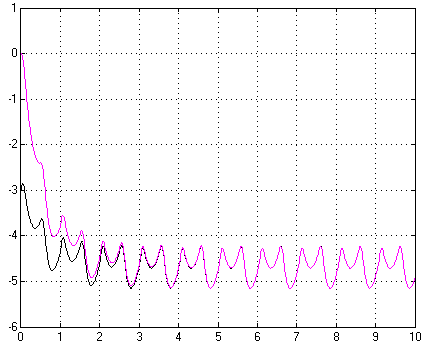
\includegraphics[width=\linewidth]{res/observer-res.png}
\caption{Observer at work.}
\label{fig:observer}
\end{figure}

After about 1,5 seconds there is only a slight difference between the two lines and after two seconds they are nearly identical. This is in agreement with the requirements for an observer; the difference $x(t)-\hat{x}$ converges to zero and after a certain time point $t_i$ where $x(t) = \hat{x}$, this equation remains satisfied for $t$\geq $t_i$.

\section*{Task 5: Controller design}

To obtain oscillatory behavior we chose the poles at $-1 + 3i$ and $-1 - 3i$. This results in the following K matrix:
\begin{equation}
\centering
K = 
\begin{bmatrix}
  0.271 & 0.168
\end{bmatrix}
\end{equation}
Leading to the oscillatory response as seen in figure \ref{fig:oscillatory}.

\begin{figure}[h!]
\centering
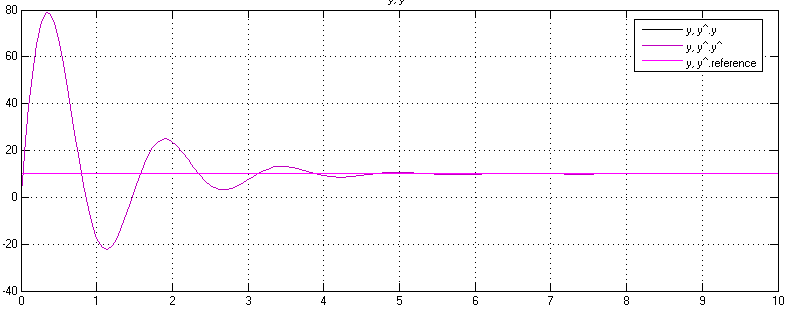
\includegraphics[scale = 0.5]{res/osc-res.png}
\caption{Oscillatory behaviour.}
\label{fig:oscillatory}
\end{figure}

To obtain the desired critically damped response we had to choose our poles in the left half-plane on the real axis. Also, they would have to be on the same exact spot, making a double pole. One would not want the poles to be too close to zero which might cause stability issues, on the other hand one would not want to place the poles too far to the left because this might not be practically feasible. Therefore the double pole was chosen at $-1.38$, which was found by trying multiple values to optimize the damping. This results in the following K matrix:
\begin{equation}
\centering
K =
\begin{bmatrix}
  -0.0641 & -0.0208
\end{bmatrix}
\end{equation}

Using this K matrix we receive a critically damped response as seen in figure \ref{fig:critically}.

\begin{figure}[H]
	\centering
    	\setlength\figureheight{4cm}
    	\setlength\figurewidth{0.8\linewidth}
    	% This file was created by matlab2tikz v0.4.6 running on MATLAB 8.3.
% Copyright (c) 2008--2014, Nico Schlömer <nico.schloemer@gmail.com>
% All rights reserved.
% Minimal pgfplots version: 1.3
% 
% The latest updates can be retrieved from
%   http://www.mathworks.com/matlabcentral/fileexchange/22022-matlab2tikz
% where you can also make suggestions and rate matlab2tikz.
% 
\begin{tikzpicture}

\begin{axis}[%
width=\figurewidth,
height=\figureheight,
scale only axis,
xmin=0,
xmax=3,
xlabel={t (s)},
ymin=0,
ymax=12,
ylabel={y},
legend style={at={(0.712050078247264,0.126460481099657)},anchor=south west,draw=black,fill=white,legend cell align=left}
]
\addplot [color=black!50!green,solid]
  table[row sep=crcr]{
0	0	\\
0.000999999999999993	0.0307620656215856	\\
0.00202035906926805	0.0620528792464848	\\
0.00304071813853609	0.0932454781366645	\\
0.00508143627707216	0.155337263841854	\\
0.00916287255414432	0.278355757838446	\\
0.0173257451082886	0.519800201126553	\\
0.0336514902165772	0.984848440945681	\\
0.0663029804331544	1.84762483116651	\\
0.115475667482295	2.99368855684154	\\
0.17051019104894	4.08640513755673	\\
0.230794632855565	5.08877982225515	\\
0.295873075612835	5.98104541793419	\\
0.365551957518053	6.75748647661367	\\
0.439792018032707	7.42042450960562	\\
0.518666908186522	7.97691474838321	\\
0.602343829925107	8.43664962788955	\\
0.691076266734968	8.8105776557425	\\
0.78520428840129	9.10998081007678	\\
0.885160600484157	9.34586327974793	\\
0.991481845317385	9.528558733129	\\
0.999999999999993	9.54076840106195	\\
1.11334367432468	9.67610444617981	\\
1.22668734864935	9.77155069484566	\\
1.35758435872145	9.84734368609818	\\
1.49758994433357	9.90080478915464	\\
1.64919825280306	9.93779744952966	\\
1.81414538231256	9.96255488496705	\\
1.99477798924578	9.97851120327929	\\
2.19408143235352	9.9883460288584	\\
2.41594910705143	9.99409201361954	\\
2.66556289595105	9.9972374567173	\\
2.94999501614365	9.99882610976487	\\
3.27919041193083	9.99955139099762	\\
};
\addlegendentry{Response};

\addplot [color=red,solid]
  table[row sep=crcr]{
0	10	\\
0.000999999999999993	10	\\
0.00202035906926805	10	\\
0.00304071813853609	10	\\
0.00508143627707216	10	\\
0.00916287255414432	10	\\
0.0173257451082886	10	\\
0.0336514902165772	10	\\
0.0663029804331544	10	\\
0.115475667482295	10	\\
0.17051019104894	10	\\
0.230794632855565	10	\\
0.295873075612835	10	\\
0.365551957518053	10	\\
0.439792018032707	10	\\
0.518666908186522	10	\\
0.602343829925107	10	\\
0.691076266734968	10	\\
0.78520428840129	10	\\
0.885160600484157	10	\\
0.991481845317385	10	\\
0.999999999999993	10	\\
1.11334367432468	10	\\
1.22668734864935	10	\\
1.35758435872145	10	\\
1.49758994433357	10	\\
1.64919825280306	10	\\
1.81414538231256	10	\\
1.99477798924578	10	\\
2.19408143235352	10	\\
2.41594910705143	10	\\
2.66556289595105	10	\\
2.94999501614365	10	\\
3.27919041193083	10	\\
};
\addlegendentry{Reference};

\end{axis}
\end{tikzpicture}%    	
    	\caption{The model’s step response with controller and observer.}
    	\label{fig:crittically}
\end{figure}

In accordance to the preceding figure we obtain the desired closed loop behaviour in our simulation.
\end{document}